\documentclass[12pt,oneside,final]{siuethesis}
\usepackage{microtype} % (optional) for more beautiful typesetting
\usepackage{graphicx} 
\usepackage{hyperref} %makes links clickable
\hypersetup{colorlinks,citecolor=black,filecolor=black,linkcolor=blue,urlcolor=black} %good for electronic copy
\hypersetup{colorlinks,citecolor=black,filecolor=black,linkcolor=black,urlcolor=black}%required for paper graduate school copy
%\usepackage[alphabetic]{amsrefs} %required if using amsrefs, comment out if using bibtex
\usepackage{fixltx2e}
\usepackage{amsmath}
\usepackage{epsf}
%\usepackage{float}
\usepackage{caption}
\usepackage{subfig}
%\usepackage{subcaption}
\usepackage{listings}
\usepackage{rotating}
\usepackage{tabularx}

\usepackage{multirow}

%% controls numbering of theorems
%% this can be configured to your advisor's taste
\newtheorem{theorem}{Theorem}[chapter] %theorem number resets each chapter
\newtheorem{conclusion}[theorem]{Conclusion}
\newtheorem{condition}[theorem]{Condition}
%% conjectures, corollary, defn, etc. numbered sequentially from beginning of chapters
\newtheorem{conjecture}[theorem]{Conjecture} 
\newtheorem{corollary}[theorem]{Corollary}
\newtheorem{example}[theorem]{Example} 
\newtheorem{lemma}[theorem]{Lemma}
\newtheorem{proposition}[theorem]{Proposition}
\newtheorem{solution}[theorem]{Solution}
\theoremstyle{definition}
\newtheorem{definition}[theorem]{Definition}


\author{Md. Monjur Ellahi Rafi}
\title{A Custom IC for Silicon Strip Detectors \protect\\
Employing the Use of Dual Shapers}

%%\advisor{John Q.\ Faculty} %% or 
\advisor{Dr.}{George L. Engel}
\secondreader{Dr.}{Bradley Noble} %% or \secondreader{Dr.}{Karl Gauss}
\thirdreader{Dr.}{Timothy York}
%\fourthreader{Karl Gauss, Sr.}
%\fifthreader{Karl Gauss, Sr.}
%\secondadvisor{Karl Gauss} %if you haves two advisors (rare) then use this line also and pass the option `twoadvisors' to the class
%\abstracttext{Chairperson: The Honorable Jill Smith} %optional -- you can use this to override the text on the abstract page; the grad school default is built-in
\submitdate{August, 2018} %date the month/year submitted to grad school, use a comma between
\copyrightyear{2016} %optional, but required if copyrighted

%% all of these are optional; defaults are shown
\major{Electrical Engineering} 
\degree{Master of Science} %can be used to specify M.A., etc.
\highestdegree{Master of Science} %used if the author already has another graduate degree
\department{Electrical and Computer Engineering} 
%\departmentname{Department}
%\refname{REFERENCES} 

%\captionsetup{width=0.7\textwidth}

\begin{document}
\maketitle 

\frontmatter %signals single spacing/roman numeral pagination

\copyrightpage %optional

%%% abstracts are optional
\begin{abstract}

This manuscript is intended to provide preliminary documentation for the sixteen channel integrated circuit (IC) under development.The  IC  is 
designed  for  use  with  an  array  of  silicon  strip  detectors  in  a  wide variety of colliding particle experiments scheduled for Fall 2002.  Only very  simple  explanations  concerning  the  operating  principles  of  the various subsystems will be provided at this time.  Emphasis is placed on simulation results predicting performance.

The  simulation  results  demonstrate  that  the  IC  will  be  capable  of providing both high resolution energy and time measurements. The IC is referred to as the HINP16C (Heavy Ion Nuclear Physics)IC throughout this 
document.  


\end{abstract}

\begin{acknowledgements}

I would like to thank Dr. George Engel, for his encouragement, support and guidance 
and also having given  me an opportunity to work with him as  his research assistant. He has 
been  a  positive  factor  in  my  academic  experience  here  at  Southern  Illinois  University, 
Edwardsville.  

I  would  like  to thank  Dr.  Lee  Sobotka  and  Mr.  Jon  Elson,  department  of  chemistry, 
Washington  University  Saint  Louis,  for  their  help  during  the  various  stages  of  this  project. 
My  special  thanks  to  the  faculty  and  staff  of  ECE  department  for  their  direct  and  indirect 
support without which I simply could not have progressed with my work. 

I am extremely grateful to Mythreyi Nethi  and Jon C.  Wade who were of great help 
during  the  entire  course  of  my  thesis  work.  I  would  also  like  to  thank  Balaji  Golla,  Arun 
Gerard and all my other friends for their constant support during my entire studies at SIUE. 

This acknowledgement would not be complete without a word of appreciation to my 
parents  and  brother  who  have  been  of  constant  encouragement  all  my  life.  Without  their 
support I would not have come so far in my life. 


\end{acknowledgements}

\tableofcontents

\cleardoublepage %cause correct numbering of list of figures

\acknowledgements

\cleardoublepage

\listoffigures %print list of figures page

\cleardoublepage

\listoftables

\mainmatter %signals single spacing/arabic numeral paginations


\chapter{INTRODUCTION}  %% chapter titles must be typed in all caps to conform with regulations



\section{Research Background}


Look at the pretty silicon strip detector array shown in Figure~\ref{FIG:HIRA_ARRAY}.

\begin{figure}[htbp!]
\centering
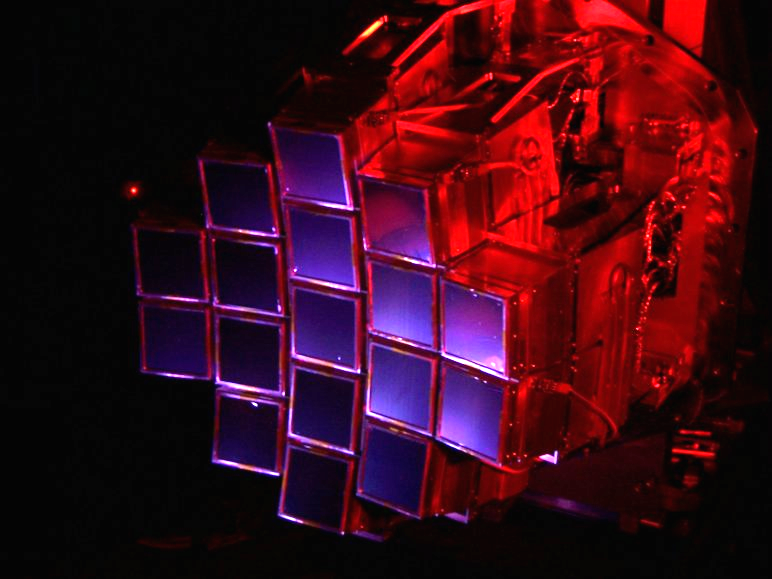
\includegraphics[scale=.6,keepaspectratio=true]{./ch1_figures/hira_array.png} 
\caption{HIRA (High-Resolution Array used at MSU)}
\label{FIG:HIRA_ARRAY}
\end{figure}



\section{Need for an Integrated Circuit}

\section{Features of HINP16C}

\section{Sample Applications}

\section{Previous work}

\section{Object and Scope of This work} 


Past experience suggests that the overall robotics platform must contain the following elements if a team is to be successful in an autonomous mobile robot competition:

\noindent
In the following section, we briefly describe the various types of motors generally encountered in robotic applications.


\section{Object and Scope of Thesis}

\chapter{HINP16C DESIGN.}


$\sqrt{x}, \omega \Omega$
\begin{equation}
x = \alpha \cdot \sqrt{x} \cdot \frac{z}{2}
\end{equation}

\begin{equation}
\Delta t_{pd}  \approx \sqrt \frac{V_{DD}}{2 \cdot \pi \cdot GBW_{c} \cdot G^N \cdot SR_{min}}
\end{equation}

\begin{equation}
\int\limits_{-\infty}^\infty k e^{-fx^2+gx+h}dx= \int\limits_{-\infty}^\infty \frac{k}{2f}e^{-f \frac{(x-g)}{(2f)}^2+g^2/(4f)+h} dx= k \sqrt{\frac{\pi}{f}} exp( \frac{g^2}{4f}+h)
\end{equation}




\section{Gaussian Equation Derivation}
Gaussian response can be described by
\begin{equation*}
h(t) = e^{-c \cdot t^2}
\end{equation*}

Taking Fourier transform of the response
\begin{equation}
|H(f)| = \sqrt{\frac{\pi}{c}} \cdot e^{\frac{- \omega ^ 2}{4 \cdot c} }
\end{equation}

Transfer function for a Gaussian filter(3rd order)
\begin{equation}
|H(f)|^2 = \frac{{\frac{\pi}{c}}} {e^{\frac{ \omega ^ 2}{2 \cdot c} }} 
\end{equation}

We want to designing a filter except the denominator should be a polynomial.

Recall that
\begin{equation}
e^x \approx 1+x+ \frac{x^2}{2!}+\frac{x^3}{3!}+\frac{x^4}{4!}+......
\end{equation}
where $x= \frac{\omega^2}{2c}$

This implies that we need an infinite order filter . We will only consider terms up to $\omega^6$ \\
Now,
\begin{align*}
|H(f)|^2&\approx \frac{\frac{\pi}{c}}{1+\frac{\omega^2}{2 \cdot c}+ \frac{1}{2} (\frac{\omega^2}{2\cdot c})^2+\frac{1}{6} (\frac{\omega^2}{2\cdot c})^3} \\
&\approx \frac{\frac{\pi}{c}}{1+\frac{\omega^2}{2 \cdot c}+ \frac{1}{8} (\frac{\omega^4}{2\cdot c^2})+ \frac{\omega^6}{48\cdot c^6}} \\
&\approx \frac{48\cdot \pi c^2}{48 c^3+24 c^2 \omega^2+6C\omega^4+\omega^6} \\
\end{align*}

Let
\begin{equation}
s=j\omega \Longrightarrow \omega= \frac{s}{j}
\end{equation}
\begin{equation}
T(s) \cdot T(-s)= \frac{48\cdot \pi c^2}{-s^6+6cs^4-24c^2s^2+48c^3}
\end{equation}
To find roots we need to set
\begin{equation}
-s^6+6cs^4-24c^2s^2+48c^3=0
\end{equation}

we use MATLAB to find the roots
\begin{equation}
s^6+0 \cdot s^5-6cs^4+0 \cdot s^3+24c^2s^2+0 \cdot s-48c^3=0 
\end{equation}
where c=1.2272



insert tonly for practice purpose Figure~\ref{FIG:RANDOM-SELECT_1}.
\begin{figure}[htbp!]
\centering
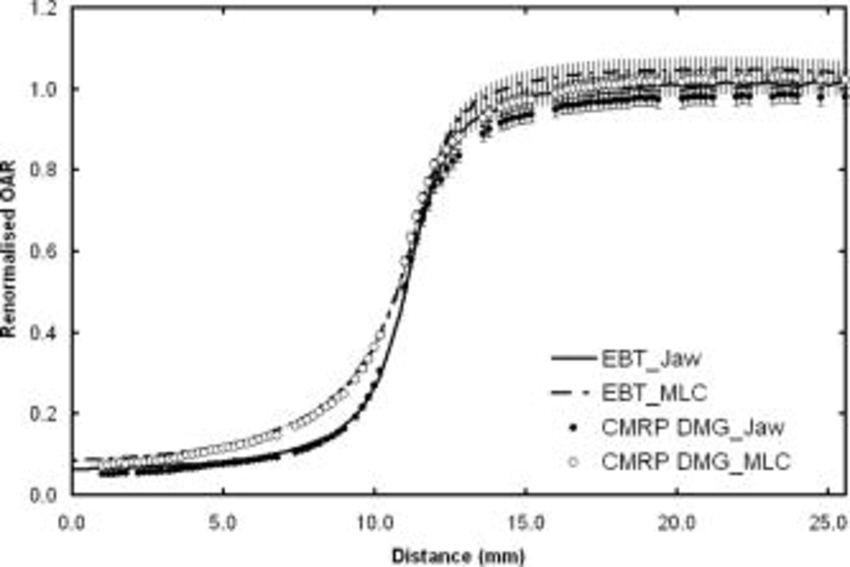
\includegraphics[scale=.4,keepaspectratio=true]{./ch2_figures/random-select_1.png} 
\caption{RANDOM (random selection for practice)}
\label{FIG:RANDOM-SELECT_1}
\end{figure}

\section{System Specifications}

\section{System Level Design}

\subsection{Linear circuits}

\subsection{Timing circuits}

\subsection{Control and read-out circuits}

\section{Charge Sensitive Amplifier (CSA)}

\subsection{Design specification of CSA}

\subsection{Design of the CSA}

\section{Pulse Shaper}

\subsection{Linear circuits}

\section{Peak Sampler}



\chapter{ELECTRICAL LEVEL DESIGN}

\section{Software Design Objectives}

silicon strip detector array shown in Figure~\ref{FIG:PACKAGED_PARTS}.
\begin{figure}[htbp!]
\centering
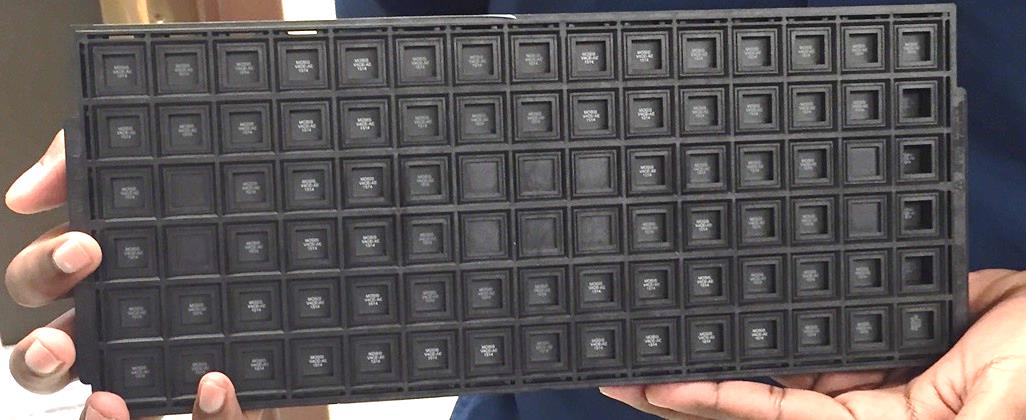
\includegraphics[scale=.4,keepaspectratio=true]{./ch3_figures/packaged_parts.png} 
\caption{Custom Chip For Use With 
Silicon Strip Detectors}
\label{FIG:PACKAGED_PARTS}
\end{figure}





\chapter{SIMULATION RESULTS}

\section{Robot Construction}
silicon strip detector array shown in Figure~\ref{FIG:INV_TER}.
\begin{figure}[htbp!]
\centering

\includegraphics[scale=0.6,keepaspectratio=true]{./ch4_figures/inverter-1.pdf} 
\caption{Custom Chip For Use With 
Silicon Strip Detectors}
\label{FIG:INV_TER}
\end{figure}





\section{PRU Library Routines}

silicon strip detector array shown in Figure~\ref{FIG:OPAMP}.
\begin{figure}[htbp!]
\centering
\includegraphics[scale=0.5,keepaspectratio=true]{./ch5_figures/op_amp.pdf} 
\caption{Custom Chip For Use With 
Silicon Strip Detectors}
\label{FIG:OPAMP}
\end{figure}


\chapter{SUMMARY, COMCLUSIONS, AND FUTURE WORK}

\section{Summary}


\section{Conclusions}

\section{Future Work}

\references %single spacing / arabic numeral paginations, adds "REFERENCES" to table of contents

%%%% for bibtex

%If you want to use bibtex  use the following lines, where your .bib file is called 'yourbib.bib'

\bibliographystyle{apalike}
\bibliography{./rafi_thesis}

% If you have only a single appendix, do it this way.

\multipleappendices
\lstset{
         language=C,
         basicstyle=\scriptsize\ttfamily,
         emptylines=0, 
         lineskip=1pt,
         %numbers=left,            
         numberstyle=\tiny,         
         stepnumber=2,              
         numbersep=5pt,             
         tabsize=3,                
         extendedchars=true,       
         breaklines=true,            
         commentstyle=\color{blue},
         keywordstyle=\color{red},
            frame=b,         
 %        keywordstyle=[1]\textbf,    
 %        keywordstyle=[2]\textbf,    
 %        keywordstyle=[3]\textbf,  
 %        keywordstyle=[4]\textbf,   \
         stringstyle=\scriptsize\color{green}\ttfamily, 
         showspaces=false,         
         showtabs=false,            
%         xleftmargin=17pt,
%         framexleftmargin=17pt,
%         framexrightmargin=5pt,
%         framexbottommargin=4pt,
         %backgroundcolor=\color{lightgray},
         showstringspaces=false           
 }


\end{document}
